\section{Experimentation}
%Describe experiments and performance measures
%Two measures of interest, time to solution and quality of solutions

We conduct a series of experiments for the noiseless and noisy simulations of our algorithm in this section. We empirically compare against the IAE and MLAE algorithms. As the update steps for these algorithms are equivalent to sampling from a Bernoulli distribution for a given choice of $\theta_0$ and noise level we sample directly from the Bernoulli distribution instead of simulating the dynamics of a quantum system for each algorithm. This algorithm has also been implemented and tested using Qiskit \cite{Qiskit}, with a view for future experiments with quantum simulators and quantum hardware.


\subsection{Simulation experiments}
\subsubsection{Noiseless experiments}
First, we explore the convergence time for a range $\theta \in [0, \pi]$. Note that as shown in \cite{callison_2022_amp_with_jitter}, so-called exceptional points occur near to rational multiples of $\pi$, therefore we sample values of $\theta$ from continuous distributions instead of equally spaced angles. Figure \ref{fig::ExAE-converge-half-circle} shows that the convergence for $\theta$ close to $0$ and $\pi$ is several orders of magnitude larger than convergence for other values. For this reason, we consider partitioning the space $\Theta = [0, \pi]$ into the central region $\Theta_0 = [\frac{\pi}{12}, \frac{11 \pi}{12}]$ and the edge region $\Theta_1 = \Theta \setminus \Theta_0 = [0, \frac{\pi}{12}) \cup (\frac{11 \pi}{12}, \pi]$

\begin{figure}[htb]
	\centering
	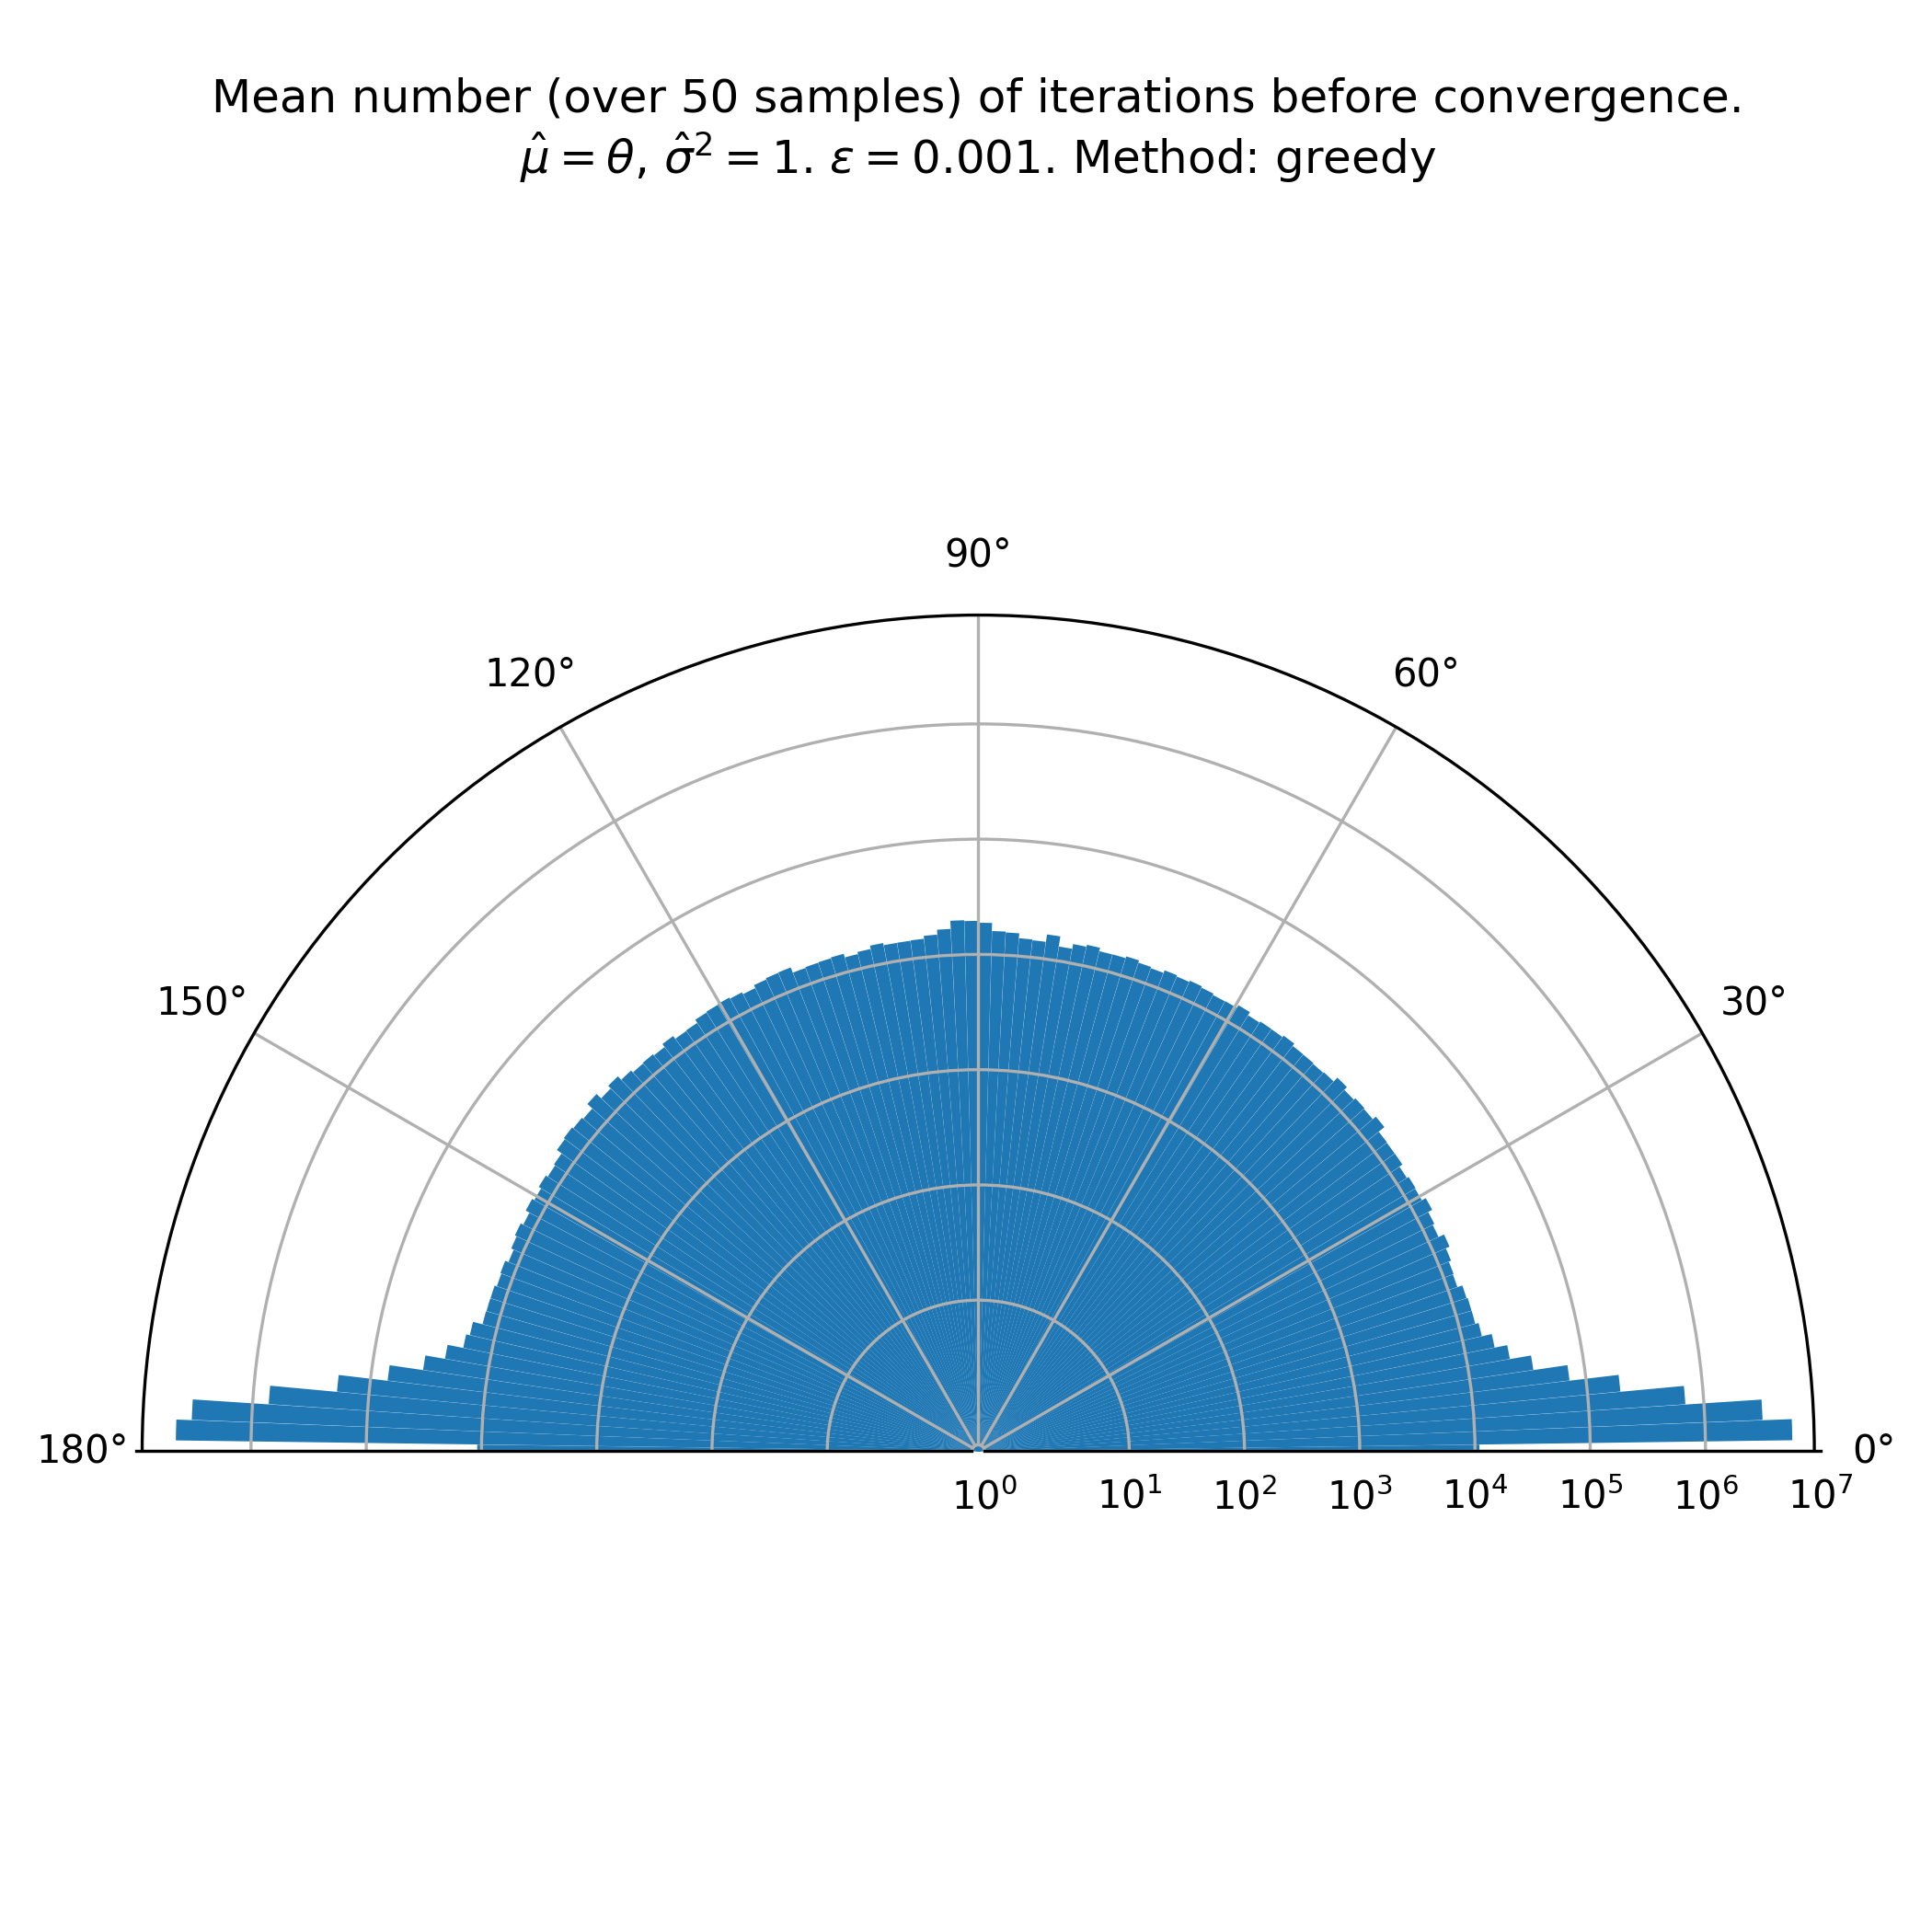
\includegraphics[scale=0.5]{ExAE-converge-half-circle}
	\caption{Median number of iterations for different error rates $\varepsilon$. Each section of the histogram is a region of width $\pi / 24$ with the median number of oracle calls calculated from 30 values of true value $\theta_0$ selected uniformly at random. The prior for each iteration is taken to be $N(\theta_0, 1)$ and success probability $1 - \alpha$ with $\alpha = 0.01$.}
	\label{fig::ExAE-converge-half-circle}
\end{figure}

\begin{itemize}
	\color{red}
	\item This should use median not mean
	\item Use radians
	\item Start with 0 on the left
	\item Should have lines for other error values
	\item Use uniform samples over each $\pi/24$ interval probably 30 samples per interval. (i.e. 720 samples total)
	\color{orange}
	\item Change $\theta$ range to $(0, \pi / 2)$ or $(0, 2 \pi)$
\end{itemize}

As seen in Figure \ref{fig::ExAE-converge-on-theta1}, the set $\Theta_1$ performs poorly for all methods that take a statistical approach. This region contains points where the variance reduction factor approach 0, with the extreme points where $\theta= 0, \frac{\pi}{2}$. 

\begin{itemize}
	\color{red}
	\item We should consider how the QoPrime and Power-law AE algorithms deal with $\Theta_1$
	\item May need a gradient graph here?
	\item Or graph of variance update ratios i.e. $\text{Var}{Y | \theta = 0} / \text{Var}{Y | \theta = 1}$ - where is this negative?
\end{itemize}


\begin{figure}[htb]
	\centering
	\caption{Median number of oracle calls for $\theta \in \Theta_1$ and fixed error rate $\varepsilon = 10^{-3}$ for different statistical amplitude estimation routines. Each section of the histogram is a region of width $\pi/120$ with the median number of oracle calls calculated from 30 values of true value $\theta_0$ selected uniformly at random. The prior for each iteration is taken to be $N(\theta_0, 1)$ and success probability $1 - \alpha$ with $\alpha = 0.01$.}
	\label{fig::ExAE-converge-on-theta1}
\end{figure}


\begin{figure}[htb]
	\centering
	\caption{Median variance for fixed error rate $\varepsilon = 10^{-3}$ against time step for $\theta_0 \in \Theta_0$ and $\theta_0 \in \Theta_1$. We sample $\theta_0$ from a uniform distribution of $x$ and $50$ samples for $\Theta_0$ and $ \Theta_1$ respectively. The prior for each iteration is taken to be $N(\theta_0, 1)$ and success probability $1 - \alpha$ with $\alpha = 0.01$.  }
	\label{fig::ExAE-var-per-step}
\end{figure}

\begin{figure}[htb]
	\centering
	\caption{Median depth for fixed error rate $\varepsilon = 10^{-3}$ against time step for $\theta_0 \in \Theta_0$ and $\theta_0 \in \Theta_1$. We sample $\theta_0$ from a uniform distribution of $x$ and $50$ samples for $\Theta_0$ and $ \Theta_1$ respectively. The prior for each iteration is taken to be $N(\theta_0, 1)$ and success probability $1 - \alpha$ with $\alpha = 0.01$.}
	\label{fig::ExAE-depth-per-step}
\end{figure}

From now on, we restrict to considering $\theta \in \Theta_0$. 

A source of potential error in this algorithm is the normal approximation made at each step. We posit that occasionally the variance decreases too fast due to this information loss, and deviates from the correct path. This can be seen in Figure, where we expect $(1-\alpha)\%$ of the points to lie above the diagonal. As a mitigation technique, we post-process the measurement data using the MLE estimator, and recover the accuracy we desire.

\begin{figure}
	\centering
	\caption{Actual precision of the final estimate for SAE with and without MLE post-processing. We sample $\theta_0 \in \Theta_0$ from a uniform distribution of $x$ and $50$ for target precisions of $\varepsilon = 10^-3, 10^-4, \ldots, 10^-7 $. The prior for each iteration is taken to be $N(\theta_0, 1)$ and success probability $1 - \alpha$ with $\alpha = 0.01$.}
	\label{fig::ExAE-actual-prec-vs-expected-prec}
\end{figure}

\begin{figure}
	\centering
	\caption{Actual precision of the final estimate for SAE with and without MLE post-processing. We sample $\theta_0 \in \Theta_0$ from a uniform distribution of $x$ and $50$ for a target precision of $\varepsilon = 10^-3$. The prior for each iteration is taken to be $N(\theta_0, 1)$ and success probability $1 - \alpha$ with $\alpha = 0.01$.}
	\label{fig::ExAE-actual-prec-over-theta}
\end{figure}

From now on, we consider selecting the depth at each step to be the minimiser of the posterior variance in an interval upper bounded by $\frac{1}{\sigma}$.
\begin{itemize}
	\color{red}
	\item Do we still need this?
	\item Should we now be throwing out the SAE by itself?
\end{itemize}

We compare the performance of ExAE to the statistical methods IAE and MLAE. 

\begin{figure}[htb]
	\centering
	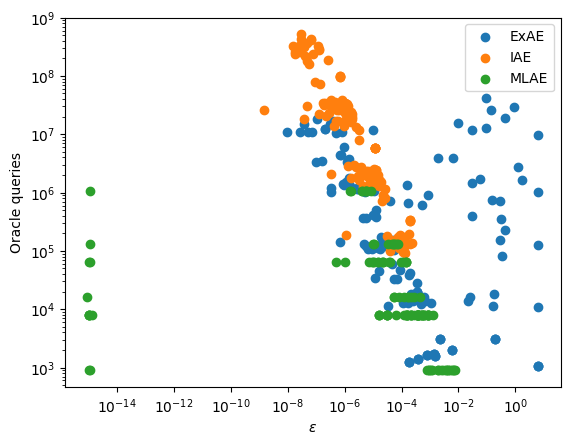
\includegraphics[scale=0.5]{query-converge-comparison}
	\caption{Final precision versus total number of oracle queries used for IAE, MLAE and ExAE. We target precisions of $\varepsilon = 10^{-3}, 10^{-4}, \ldots , 10^{-7}$, with each point a single value of $\theta_0 \in \Theta_0$. We sample uniformly from $\Theta_0$ for 30 values of $\theta_0$. Each value of $\theta_0$ is evaluated for all algorithms and each target $\varepsilon$. The prior for each iteration is taken to be $N(\theta_0, 1)$ and success probability $1 - \alpha$ with $\alpha = 0.01$.}
	\label{fig::query-comparison-noiseless}
\end{figure}


\begin{figure}[htb]
	\centering
	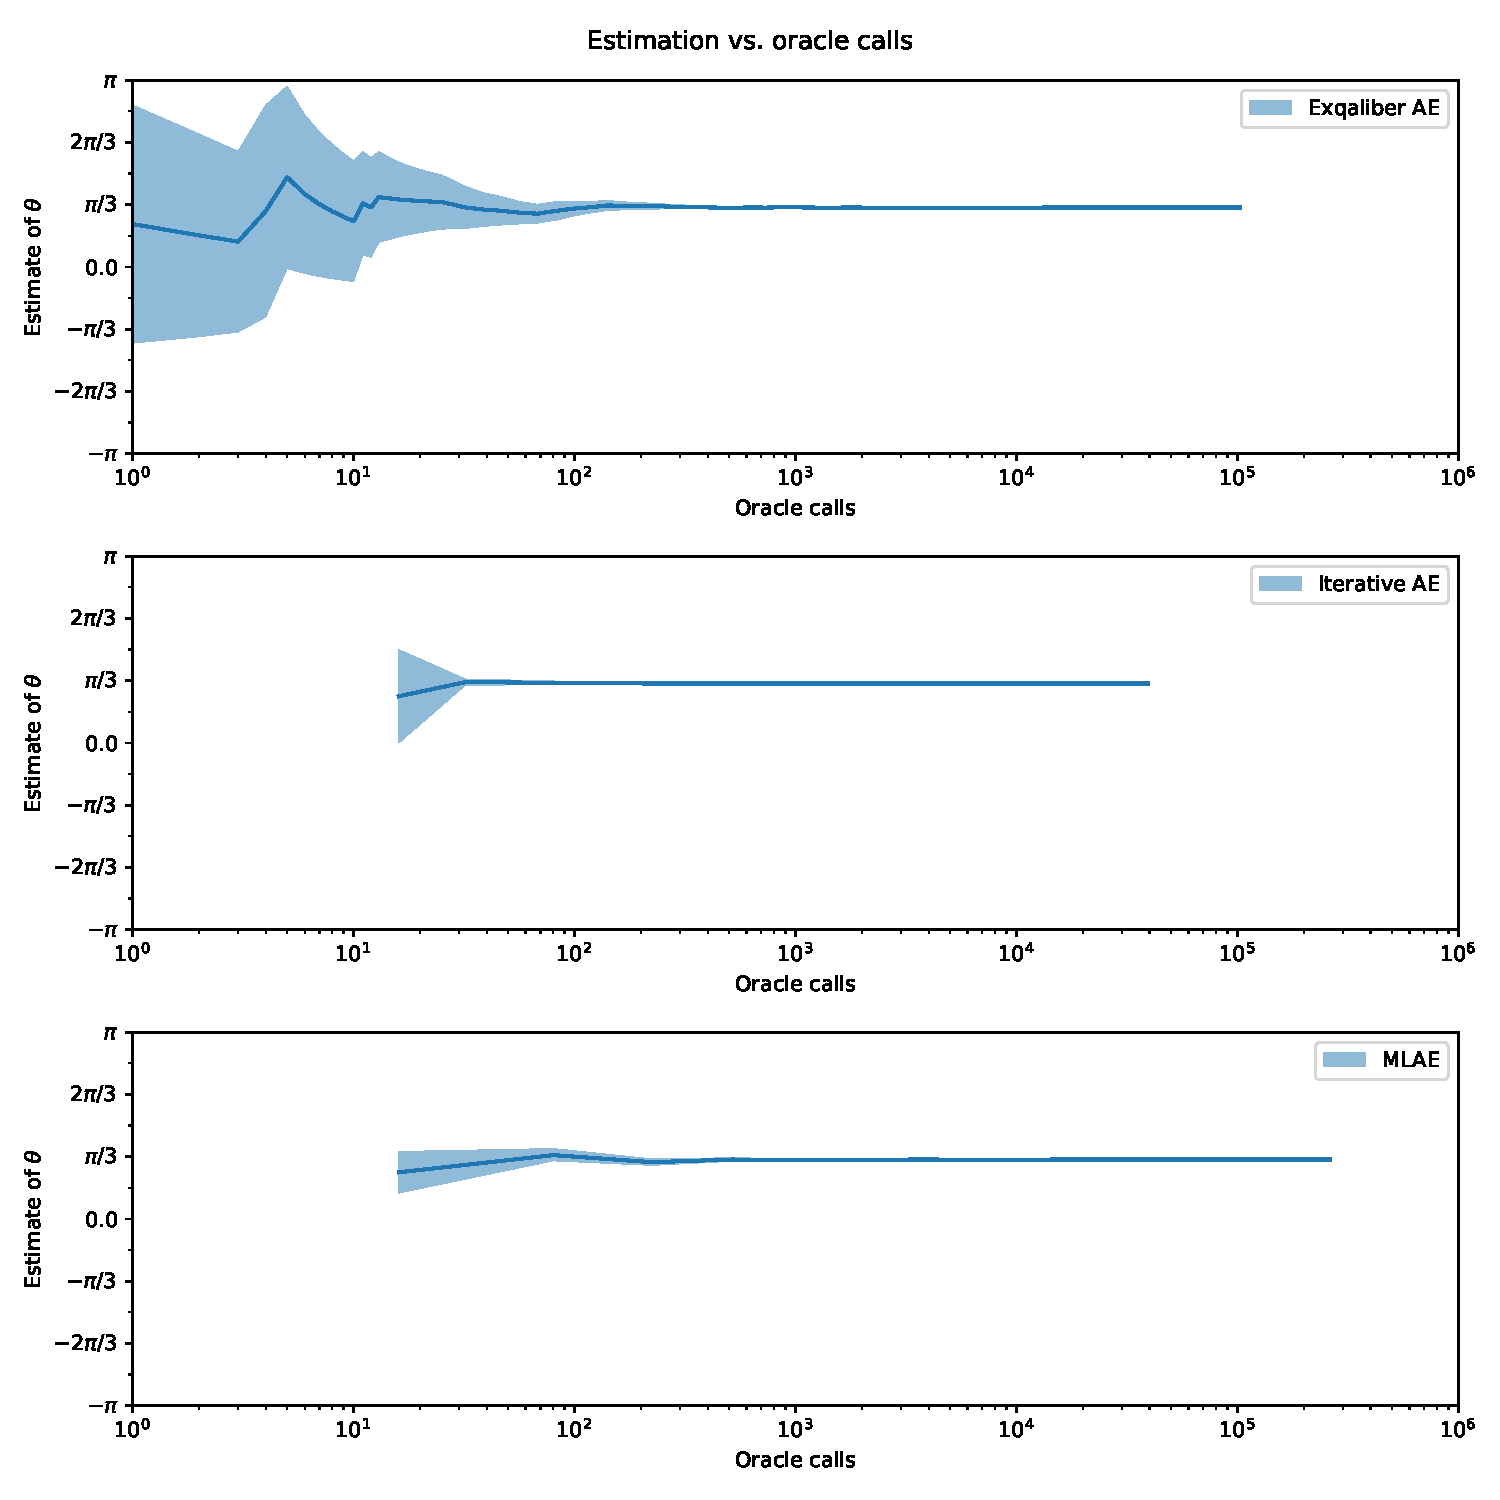
\includegraphics[scale=0.5]{compare-paths-oracle-calls}
	\caption{Confidence intervals for a single run of Canonical AE, IAE, MLAE and ExAE with $\theta = \pi / 2$. The prior for ExAE is taken to be $N(\pi/2, 1)$ and success probability $1 - \alpha$ with $\alpha = 0.01$.}
	\label{fig::compare-paths-oracle-calls}
\end{figure}

\subsubsection{Decoherence noise experiments}

We explore the performance of our algorithm for a range of noise rates.

As shown in Figure \ref{fig::ExAE-noisy-max-depth}, the algorithm will not go beyond a depth of $\sim \frac{1}{\lambda}$. 

\begin{itemize}
	\color{red}
	\item Should have a graph of posterior distribution for different error rates. 
\end{itemize}

\begin{figure}[htb]
	\centering
	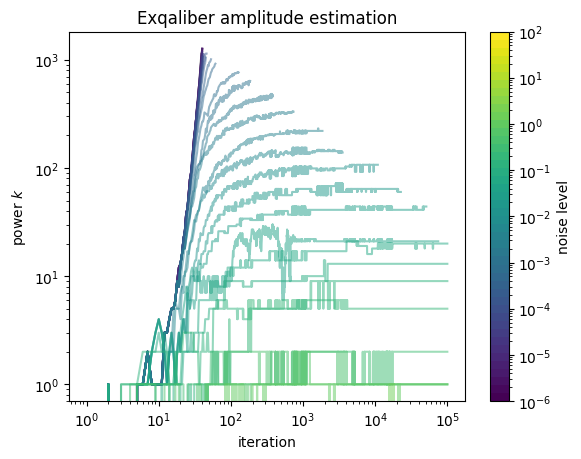
\includegraphics[scale=0.5]{ExAE-noisy-max-depth}
	\caption{Depth of ExAE for $\theta_0 = \pi / 2$ at varying levels of decohering noise characterised by $\lambda = 10^0, 10^{-1}, \ldots 10^{-6}$. The prior for each iteration is taken to be $N(\pi /2, 1)$, we target $\varepsilon = 10^{-3}$ and success probability $1 - \alpha$ with $\alpha = 0.01$.}
	\label{fig::ExAE-noisy-max-depth}
\end{figure}

\begin{figure}[htb]
	\centering
	\caption{Total number of oracle queries for ExAE with decohering noise characterised by $\lambda = 10^{-1}, 10^{-2}, \ldots, 10^{-7}$. Each point is a single value of $\theta_0 \in \Theta_0$. We sample uniformly from $\Theta_0$ for 30 values of $\theta_0$. Each value of $\theta_0$ is evaluated for all decohering noise values and each target $\varepsilon$. The prior for each iteration is taken to be $N(\theta_0, 1)$ and success probability $1 - \alpha$ with $\alpha = 0.01$.}
	\label{fig::query-exae-noisy}
\end{figure}

\begin{itemize}
	\color{red}
	\item Concerned that error comparisons make no sense here. These algorithms have no capacity to cope with noise so obviously they're bad - but others e.g. Hitachi, QoPrime, Power-law AE do
\end{itemize}

\begin{figure}[htb]
	\centering
	\caption{Final precision versus total number of oracle queries used for IAE, MLAE and ExAE with decohering noise characterised by $\lambda = 10^{-3}$. We target precisions of $\varepsilon = 10^{-3}, 10^{-4}, \ldots , 10^{-7}$, with each point a single value of $\theta_0 \in \Theta_0$. We sample uniformly from $\Theta_0$ for 30 values of $\theta_0$. Each value of $\theta_0$ is evaluated for all algorithms and each target $\varepsilon$. The prior for each iteration is taken to be $N(\theta_0, 1)$ and success probability $1 - \alpha$ with $\alpha = 0.01$.}
	\label{fig::query-comparison-noisy}
\end{figure}




%% This is probably explained earlier, but I need it for my argument, so I wrote it. In the final version, we probably need to refer to earlier in the text.
%In amplitude estimation, there is an operator $\mathcal{A}$ acting on $n+1$ qubits, such that $\mathcal{A} \ket{\psi}_{n+1} = \sqrt{a}\ket{\psi_1}_{n}\ket{1} + \sqrt{1-a}\ket{\psi_0}_n\ket{0}$,
%with $a\in [0,1]$ or, when defining $a=\sin^2{\theta_a}$ with $\theta_a \in [0, \pi]$,
%\begin{equation}
%	\mathcal{A}_{n+1} \ket{\psi} = \sin{\theta_a} \ket{\psi_1}_n \ket{1}
%	+ \cos{\theta_a}\ket{\psi_0}_n\ket{0}.
%\end{equation}
%The goal is to find $\theta_a$.
%
%One can create an operator $\mathcal{Q} = \mathcal{A} \mathcal{S}_0 \mathcal{A}^{\dagger}\mathcal{S}_{\psi_0}$ with $\mathcal{S}_{\psi_0} = \mathbb{I} - 2\ket{\psi_0}_n\bra{\psi_0}_n\otimes\ket{0}\bra{0}$ and $\mathcal{S}_0 = \mathbb{I} - 2\ket{0}_{n+1}\bra{0}_{n+1}$. % TODO reference
%% TODO choose definition of 'oracle queries'. In the iterative AE paper, they "denote applications of Q as quantum samples or oracle queries."
%Now by applying $\mathcal{Q}$ for $k$ times (and thereby applying $\mathcal{A}$ a total of $(2k+1)$ times), the probability of measuring the $\ket{1}$ state follows a Bernoulli distribution with $p$ equal to
%\begin{equation}
%	p = \frac{1}{2}(1-\cos{((2k+1)\theta_a)}).
%	\label{eq:bernoulli-p}
%\end{equation}
%Using this equation, one can test different amplitude estimation analytically, by sampling from the Bernoulli distribution directly. We call this direct analytical sampling.
%
%We experimented with our novel amplitude estimation routine. There are two relevant measures for amplitude estimation.
%These are the time to solution (and its scaling) and the quality of the solution, i.e., the error $\epsilon$.
%To measure these, we simulate experiments using direct analytical sampling.
%
%
%As our algorithm uses dynamical updates, depending on the true $\theta$, %TODO: make this consistent throughout the article. Maybe theta hat?
%anomalies can rise for values around integer fractions of $\pi$.
